% Template for a Computer Science Tripos Part II project dissertation
\documentclass[12pt,a4paper,twoside,openright]{report}
\usepackage[pdfborder={0 0 0}]{hyperref}    % turns references into hyperlinks
\usepackage[margin=25mm]{geometry}  % adjusts page layout
\usepackage{graphicx}  % allows inclusion of PDF, PNG and JPG images
\usepackage{verbatim}
\usepackage{docmute}   % only needed to allow inclusion of proposal.tex
\usepackage{tikz}
\usetikzlibrary{shapes.geometric, arrows}
\usepackage{multirow}
\usepackage{url}
\usepackage{csquotes}

\raggedbottom                           % try to avoid widows and orphans
\sloppy
\clubpenalty1000%
\widowpenalty1000%

\renewcommand{\baselinestretch}{1.1}    % adjust line spacing to make
                                        % more readable

\begin{document}

\bibliographystyle{plain}


%%%%%%%%%%%%%%%%%%%%%%%%%%%%%%%%%%%%%%%%%%%%%%%%%%%%%%%%%%%%%%%%%%%%%%%%
% Title


\pagestyle{empty}

\rightline{\LARGE \textbf{Simonas Mulevicius}}

\vspace*{60mm}
\begin{center}
\Huge
\textbf{QUIC offloading using NetFPGA smart NICs} \\[5mm]
Computer Science Tripos -- Part II \\[5mm]
Homerton College \\[5mm]
\today  % today's date
\end{center}

%%%%%%%%%%%%%%%%%%%%%%%%%%%%%%%%%%%%%%%%%%%%%%%%%%%%%%%%%%%%%%%%%%%%%%%%%%%%%%
% Proforma, table of contents and list of figures

\pagestyle{plain}

\chapter*{Proforma}

{\large
\begin{tabular}{ll}
Name:               & \bf Simonas Mulevicius                       \\
College:            & \bf Homerton College                     \\
Project Title:      & \bf QUIC offloading using NetFPGA smart NICs \\
Examination:        & \bf Computer Science Tripos -- Part II, July 2021  \\
Word Count:         & \bf 2282\footnotemark[1] \\
Project Originator: & Dr Andrew W. Moore                \\
Supervisor:         & Dr Andrew W. Moore                \\ 
\end{tabular}
}
\footnotetext[1]{This word count was computed
by \texttt{DISS\_LENGTH=\$(detex diss.tex | tr -cd '0-9A-Za-z $\tt\backslash$n' | wc -w); PROPOSAL\_LENGTH=\$(detex proposal.tex | tr -cd '0-9A-Za-z $\tt\backslash$n' | wc -w); echo "\$((\$DISS\_LENGTH-\$PROPOSAL\_LENGTH))"}}

\stepcounter{footnote}


\section*{Original Aims of the Project}

TODO

\section*{Work Completed}

TODO

\section*{Special Difficulties}

TODO
 
\newpage
\section*{Declaration}

I, Simonas Mulevicius of Homerton College, being a candidate for Part II of the Computer
Science Tripos, hereby declare
that this dissertation and the work described in it are my own work,
unaided except as may be specified below, and that the dissertation
does not contain material that has already been used to any substantial
extent for a comparable purpose. I am content for my dissertation to
be made available to the students and staff of the University.

\bigskip
\leftline{Signed [signature]}

\medskip
\leftline{Date [date]}


%Professional Practice and Presentation 14%
%Introduction and Preparation 26%
%Implementation 40%
%Evaluation and Conclusion 20%




\tableofcontents

\listoffigures

\newpage
\section*{Acknowledgements}

The following people helped with the project setup or provided useful insights or hints on how to tackle project-related problems:
\begin{itemize}
    \item \textbf{Dr Marcin Wojcik} helped with general inquiries related to the setup of NetFPGA developing platform;
    \item \textbf{Dr Andrew W. Moore} was my project supervisor and originator of the project idea;
    \item \textbf{Dr Malcolm Scott} helped with the configuration of two remote backup machines in the Computer Laboratory that were used for experiments during the Winter vacation;
    \item \textbf{Mr Tatsuhiro Tsujikawa} is the author of \texttt{ngtcp2}\footnote{specific implementation of QUIC which is used in this project}, and he answered usability questions related to it. Moreover, he provided guidance on how null encryption could be turned on in \texttt{ngtcp2}.
\end{itemize}

Furthermore, this document is written using a default dissertation template provided by Martin Richards \cite{how_to_write_a_dissertation_in_LATEX}.
However, some formatting ideas are taken from Alex Coplan's dissertation \cite{Alex_Coplan_dissertation}, which, according to \cite{Computer_Lab_dissertations}, is \enquote{highly commended by the examiners}.

%%%%%%%%%%%%%%%%%%%%%%%%%%%%%%%%%%%%%%%%%%%%%%%%%%%%%%%%%%%%%%%%%%%%%%%
% now for the chapters

\pagestyle{headings}

\chapter{Introduction}
% ------------------------------------------------
% TODO
%
% The introduction should explain the principal motivation for the project and show how the work fits into the broad area of surrounding computer science and give a brief survey of previous related work. It should generally be unnecessary to quote at length from technical papers or textbooks. If a simple bibliographic reference is insufficient, consign any lengthy quotation to an appendix.



% FROM: https://www.cst.cam.ac.uk/teaching/part-ii/projects/assessment
% Clear motivation, justifying potential benefits of success.
%Good or excellent requirements analysis; justified and documented selection of suitable tools; good engineering approach.
%Clear presentation of challenging background material covering a range of computer science topics beyond Part IB.
% ------------------------------------------------


\section{What is \texttt{QUIC?}}

\texttt{QUIC} is a next-generation transport layer protocol built on top of UDP \cite{chromium_blog_about_quic}.
Figure~\ref{fig:QUIC_network_stack} shows the network stack of QUIC.

    \begin{figure}[h]
    \centering
    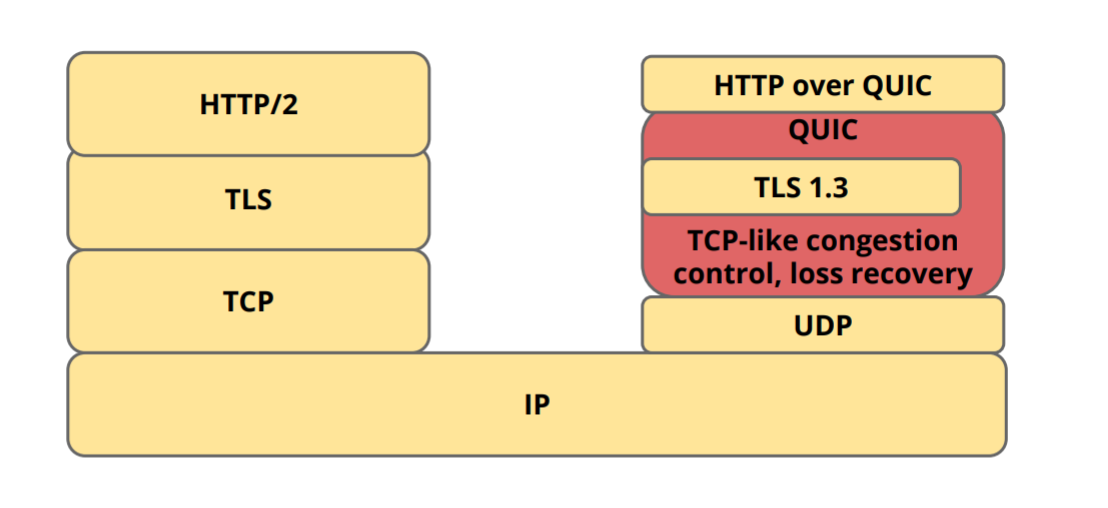
\includegraphics[width=0.9\textwidth]{figs/QUIC_network_stack.PNG}
    \caption{QUIC/UDP/IP network stack compared to TCP/IP network stack. This diagram is taken from IETF presentation about QUIC \cite{IETF_presentation_about_QUIC}.}
    \label{fig:QUIC_network_stack}
    \end{figure}

% [TODO: WHAT end-to-end LATENCY?]
One of the key ideas of QUIC is that it aims to reduce end-to-end latency by combining handshakes of both transport (\texttt{QUIC}) and security (\texttt{TLS1.3}) layers \cite{Google_QUIC_protocol_moving_the_web_from_TCP_to_UDP}, \cite{HTTP_3_the_past_the_present_and_the_future}. Hence, for this reason \texttt{TLS1.3} layer in Figure~\ref{fig:QUIC_network_stack} is shown as being part of the QUIC protocol. 
As Mattias Geniar said \cite{Google_QUIC_protocol_moving_the_web_from_TCP_to_UDP},
\texttt{HTTP over QUIC} layer (which is called \texttt{HTTP/3} \cite{HTTP_3_the_past_the_present_and_the_future}) is smaller than analogous \texttt{HTTP/2} layer because stream multiplexing and connection management tasks are delegated to QUIC.
Similarly, the UDP layer is smaller than the TCP layer because UDP does not provide congestion control. 
In other words, UDP sends packets in \enquote{fire and forget} manner \cite{Google_QUIC_protocol_moving_the_web_from_TCP_to_UDP}.


\subsection{List of QUIC Features}
% https://archive.nanog.org/sites/default/files/meetings/NANOG64/1051/20150603_Rogan_Quic_Next_Generation_v1.pdf
\begin{itemize}
  \item TODO congestion control
  \item TODO loss detection with signaling (using new seq number)
  \item TODO loss recovery
  \item TODO reliability
  \item TODO multiplexed streams
  \item TODO connection migration (https://peering.google.com/\#/learn-more/quic, https://ma.ttias.be/googles-quic-protocol-moving-web-tcp-udp/)
  \item TODO encryption by default
  \item TODO Mention fast TLS1.3 handshake
  \item TODO mention zero RTT handshake
\end{itemize}


%  TODO So what are those problems?! 
\subsection{\texttt{HTTP/1.0} Problems caused by \texttt{TCP}}
\texttt{QUIC} aims to solve some of the design problems which are present in the \texttt{TCP} transport layer protocol.
As Charles M. Kozierok states in his book \cite{TCP_IP_Guide_Book},
\texttt{HTTP/1.0} suffers from the fact that it uses one \texttt{TCP} connection for every \texttt{HTTP} request-reply pair. 
A similar idea is expressed in the article written by Alessandro Ghedini and Rustam Lalkaka
\cite{HTTP_3_the_past_the_present_and_the_future}.
Opening a new \texttt{TCP} connection for every small web object causes \texttt{TCP} to be constantly in the \enquote{slow start} phase, meaning that small files usually are not sent at the peak throughput \cite{HTTP_3_the_past_the_present_and_the_future}.
Furthermore, \texttt{HTTP/1.0} suffers from the fact that for every request it needs to complete \texttt{TCP} and \texttt{TLS} handshakes, which in turn can take several round-trip times to complete \cite{HTTP_3_the_past_the_present_and_the_future}.


\subsection{Previous Attempts to Improve \texttt{TCP} by Using \texttt{HTTP/1.1} and \texttt{SPDY}}

[TODO describe \texttt{HTTP/1.1}]
% TODO: According https://www.oreilly.com/content/will-http2-make-my-site-faster/, HTTP/1.1 uses six TCP connections



[TODO describe \texttt{SPDY}]



% TODO also, add references!
There have already been several attempts to overcome the head-of-line blocking problem present in TCP.
However, attempts to roll out new and experimental versions of TCP were unsuccessful. 
%TODO justify - mention SPDY and TCP.2??
The main reason being that middleboxes (e.g. Network Address Translators or NATs for short) interfered with the TCP traffic.
For instance, NATs made assumptions about the structure of TCP headers.
As TCP/IP stack was and still is a predominant backbone of the Internet, some NATs offloaded some TCP processing to hardware or used some software optimisation techniques.
Consequently, these premature optimisations interfered with TCP protocol's correctness - NATs rejected connections that used experimental TCP packets.
Another reason for the slow roll-out was that TCP's functionality is implemented in the kernel, meaning that in order to add changes to TCP, one would need to change a large number of different operating systems.
Architects of QUIC learned these mistakes and attempted to prevent the ossification of QUIC in the future by using two interesting techniques.
To simplify the deployment, QUIC's code operates in userspace.
In addition, to prevent NATs from interfering with QUIC, QUIC's packet headers are partially encrypted (see subsection \ref{subsection_QUIC_header_format}).




\subsection{\texttt{QUIC}'s Advantages}

\begin{itemize}
  \item Reduced latency:
  According to [https://blog.chromium.org/2015/04/a-quic-update-on-googles-experimental.html]: "$<\ldots>$ QUIC outshines TCP under poor network conditions, shaving a full second off the Google Search page load time for the slowest 1\% of connections".
  \item TODO mention head-of-line blocking
  \item TODO mention combined handshake protocol 
  % TODO: read https://blog.cloudflare.com/introducing-0-rtt/
  
  \item TODO mention how QUIC solves the problem of ossification
\end{itemize}

\subsection{\texttt{QUIC}'s Header Format} \label{subsection_QUIC_header_format}

\begin{itemize}
  \item TODO mention that the packet header encryption is separate from payload encryption
  \item TODO explain why do we need this separation
  \item TODO present long and short headers give a list of fields
  \item TODO mention that packet numbers are encrypted, but connection ID is not
\end{itemize}


\subsection{\texttt{QUIC}'s Adoption}

At the time of writing, $5.0\%$ of all the websites on the Internet used \texttt{QUIC} and $14.5\%$ used \texttt{HTTP/3} \cite{bib_Adoption_comparison_Between_http2_http3_quic}
(see Figure~\ref{fig:Adoption_comparison_Between_http2_http3_quic}).

    \begin{figure}[h]
    \centering
    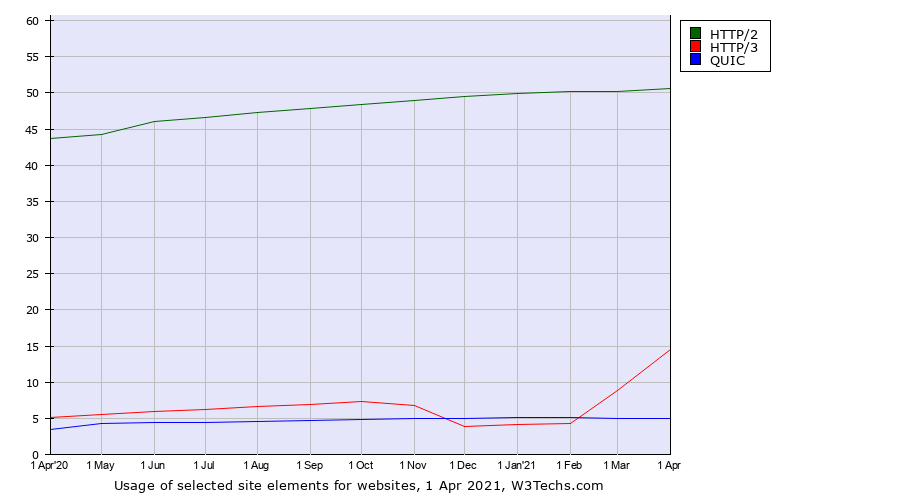
\includegraphics[width=0.9\textwidth]{figs/Adoption_comparison_Between_http2_http3_quic.png}
    \caption{Proportion of websites using \texttt{QUIC}, \texttt{HTTP/2} or \texttt{HTTP/3}. This diagram is taken from \cite{bib_Adoption_comparison_Between_http2_http3_quic}.}
    \label{fig:Adoption_comparison_Between_http2_http3_quic}
    \end{figure}



\section{Related Work}
\subsection{TODO: give an overview of Gianni's paper}



% \section{Number of words}
% TODO TO USE

% An approximate word count of the body of the dissertation may be
% obtained using:

% \texttt{wc diss.tex}

% \noindent
% Alternatively, try something like:
% \verb/detex diss.tex | tr -cd '0-9A-Z a-z\n' | wc -w/


\chapter{Preparation}
% ------------------------------------------------
% TODO
%
% Principally, this chapter should describe the work which was undertaken before code was written, hardware built or theories worked on. It should show how the project proposal was further refined and clarified, so that the implementation stage could go smoothly rather than by trial and error.

%Throughout this chapter and indeed the whole dissertation, it is essential to demonstrate that a proper professional approach was employed.

%The nature of this chapter will vary greatly from one dissertation to another but, underlining the professional approach, this chapter will very likely include a section headed "Requirements Analysis" and refer to appropriate software engineering techniques used in the dissertation. The chapter will also cite any new programming languages and systems which had to be learnt and will mention complicated theories or algorithms which required understanding.

%It is essential to declare the starting point. This states any existing codebase or materials that your project builds on. The text here can commonly be identical to the text in your proposal, but it may enlarge on it or report variations. For instance, the true starting point may have turned out to be different from that declared in the proposal and such discrepancies must be explained.



% FROM: https://www.cst.cam.ac.uk/teaching/part-ii/projects/assessment
% Clear motivation, justifying potential benefits of success.
%Good or excellent requirements analysis; justified and documented selection of suitable tools; good engineering approach.
%Clear presentation of challenging background material covering a range of computer science topics beyond Part IB.
% ------------------------------------------------




\section{Implementations of QUIC}

\subsection{List of QUIC's Implementations} \label{List_of_QUIC_implementations}
According to QUIC Working Group \cite{number_of_QUIC_implementations}, there is 31 different implementation of QUIC. Most of the implementations, 22 to be precise, are written using C/C++ language family (e.g. \texttt{Chromium}\footnote{https://chromium.googlesource.com/chromium/src/net/+/master/quic/}) while remaining implementations use Rust (e.g. \texttt{quiche}\footnote{https://github.com/cloudflare/quiche}), Python (e.g. \texttt{aioquic}\footnote{https://github.com/aiortc/aioquic}), Haskel (e.g. \texttt{Haskell quic}\footnote{https://github.com/kazu-yamamoto/quic}), Java (e.g. \texttt{kwik}\footnote{https://bitbucket.org/pjtr/kwik/src/master/}), Go (e.g. \texttt{quic-go}\footnote{https://github.com/lucas-clemente/quic-go}) or JavaScript (e.g. \texttt{Node.js QUIC}\footnote{https://github.com/nodejs/quic}).


\subsection{Why are there so many Implementations of QUIC?}

% TODO user space vs kernel space

As I have already mentioned in the Introduction section, QUIC is implemented in the user space [TODO ADD SOURCE].


\subsection{Why did I choose  \texttt{ngtcp2}?}
%TODO: fix style and grammar:
There are many implementations of QUIC (see subsection \ref{List_of_QUIC_implementations}) written in different languages.
I considered  \texttt{aioquic}\footnote{https://github.com/aiortc/aioquic},  \texttt{MsQuic}\footnote{https://github.com/microsoft/msquic},  \texttt{ngtcp2}\footnote{https://github.com/ngtcp2/ngtcp2},  \texttt{mvfst}\footnote{https://github.com/facebookincubator/mvfst} and \texttt{Quant}\footnote{https://github.com/NTAP/quant}.
One of the primary goals of the project was to turn off header encryption of QUIC packets.
% TODO mention why I needed to turn off header encryption in the first place
Hence, I performed a survey to find QUIC implementation, which had an API to control encryption. 
\texttt{Aioquic}, \texttt{MsQuic} and \texttt{ngtcp2} seemed to be the most promising.
However, despite being a simple and well-documented implementation of QUIC, aioquic did not have an active development team that could answer technical questions.
Similarly, MsQuic seemed promising, but some of the performance measurement tools used by the MsQuic team were proprietary and not yet released to the public.
As this project is based on a paper written by Gianni Antichi and his colleagues \cite{Making_QUIC_Quicker}, I thought that it would be wise to use similar testing conditions in this dissertation too.
In particular, Gianni and his team evaluated several QUIC implementations, which were written in C or C++.
Hence, I decided to follow a similar approach, and I picked \texttt{ngtcp2}, which is also written in C.
Later on, I figured out that there is an experimental QUIC benchmarking tool called \texttt{h2load}\footnote{https://github.com/nghttp2/nghttp2/tree/quic}, which is compatible with \texttt{ngtcp2}.
Moreover, \texttt{h2load} is written by Mr Tatsuhiro  Tsujikawa (the co-author of \texttt{ngtcp2}).


\section{Requirements Analysis}

\section{Starting Point}
As mentioned in the previous sections, this project builds on top of \texttt{ngtcp2} implementation of \texttt{QUIC}.
In other words, relevant networking stack tools such as cryptographic library (e.g. \texttt{OpenSSL}), benchmarking tool (e.g. \texttt{h2load}), custom \texttt{HTTP} layers (e.g. \texttt{nghttp2} and \texttt{ngtcp3}) have already been built and integrated. 
Similarly, the concept of QUIC was introduced in the Part IB \enquote{Computer Networking} course and fundamentals of C and C++ were covered in \enquote{Programming in C and C++} course. 
In addition, I used C++11 in my summer internship.


\chapter{Implementation}
% ------------------------------------------------
% TODO

%This chapter should describe what was actually produced: the programs which were written, the hardware which was built or the theory which was developed. Any design strategies that looked ahead to the testing stage should be described in order to demonstrate a professional approach was taken.

%Descriptions of programs may include fragments of high-level code but large chunks of code are usually best left to appendices or omitted altogether. Analogous advice applies to circuit diagrams or detailed steps in a machine-checked proof.

%The implementation chapter should include a section labelled "Repository Overview". The repository overview should be around one page in length and should describe the high-level structure of the source code found in your source code repository. It should describe whether the code was written from scratch or if it built on an existing project or tutorial. Making effective use of powerful tools and pre-existing code is often laudable, and will count to your credit if properly reported. Nevertheless, as in the rest of the dissertation, it is essential to draw attention to the parts of the work which are not your own. 

%It should not be necessary to give a day-by-day account of the progress of the work but major milestones may sometimes be highlighted with advantage.


% FROM: https://www.cst.cam.ac.uk/teaching/part-ii/projects/assessment
%Contribution to the field.
%Application of extra-curricular reading and original interpretation of previous work from academia or industry.
%Challenging goals and substantial deliverables with excellent selection and application of appropriate mathematical, scientific and/or engineering techniques.
%Clear and justified repository overview.
%At most minor faults in execution or understanding.
% ------------------------------------------------

\section{Repository Overview} 
% TODO add reference to the original page of ngtcp2
First of all, I added support of null encryption in the cloned repository of \texttt{ngtcp2}.

\section{Using Null Encryption}
% TODO add reference that encryption is turned on by default
By design, QUIC uses encryption by default.
It encrypts both the payloads of the packets and some fields in the packet headers.
% TODO add a reference showing that QUIC crypto functions are expensive
However, encryption and decryption operations were found to be computationally expensive.
These intensive operations could have become a performance bottleneck of QUIC.
To validate this claim, I had to measure the impact of cryptographic operations on QUIC's performance by comparing the throughput between the two server-client pairs.
One pair had to use standard encryption and decryption procedures, while another had to exchange unencrypted packets.
I achieved this by implementing logic that can turn on null encryption on \texttt{ngtcp2}.
% TODO add a link to null encryption
In essence, null encryption is a technique that effectively turns off encryption by encrypting/decrypting the data by ``XOR"ing the data with a key made entirely of zeroes (which leaves the data unchanged). 


% TODO - say which operations are performed and which ones are omitted






\chapter{Evaluation}
% ------------------------------------------------
%This is where Assessors will be looking for signs of success and for evidence of thorough and systematic evaluation. Sample output, tables of timings and photographs of workstation screens, oscilloscope traces or circuit boards may be included. Care should be employed to take a professional approach throughout. For example, a graph that does not indicate confidence intervals will generally leave a professional scientist with a negative impression. As with code, voluminous examples of sample output are usually best left to appendices or omitted altogether.

%There are some obvious questions which this chapter will address. How many of the original goals were achieved? Were they proved to have been achieved? Did the program, hardware, or theory really work?

%Assessors are well aware that large programs will very likely include some residual bugs. It should always be possible to demonstrate that a program works in simple cases and it is instructive to demonstrate how close it is to working in a really ambitious case.
% ------------------------------------------------



\section{Setup}

As this project builds on the ideas presented in \cite{Making_QUIC_Quicker}, I thought that it would be reasonable to replicate a similar testing environment to obtain comparable results.

\subsection{Logical Setup}
To test a simple single flow performance, it is sufficient to have a single QUIC server-client pair, as depicted in Figure~\ref{fig:Logical_testing_environment}.
To measure QUIC performance under different conditions, we need to add a network emulator between the QUIC client and the QUIC server.

    \begin{figure}[h]
    \centering
    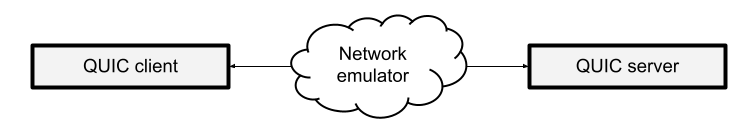
\includegraphics[width=0.9\textwidth]{figs/Logical_testing_environment.png}
    \caption{Logical configuration of testing environment}
    \label{fig:Logical_testing_environment}
    \end{figure}

\subsection{Physical Setup}
    In the ideal scenario, we might want to use three dedicated machines for performance measurements, as shown in the previous section.
    However, I decided to use a slightly different physical layout (see Figure~\ref{fig:Physical_testing_environment}).
    In this environment, one machine (A) hosts client-server pair, while another computer (B) acts as a network emulator.
    The physical configuration differs from the logical configuration because I wanted to replicate testing conditions under which Gianni Antichi and his colleagues performed throughput measurements of QUIC \cite{Making_QUIC_Quicker}.
    One advantage of having both server and client running on the same machine is that the shared system clock can perform measurements more accurately. 
    
% TODO mention that the diagram was taken from Gianni's paper
    \begin{figure}[ht]
    \centering
    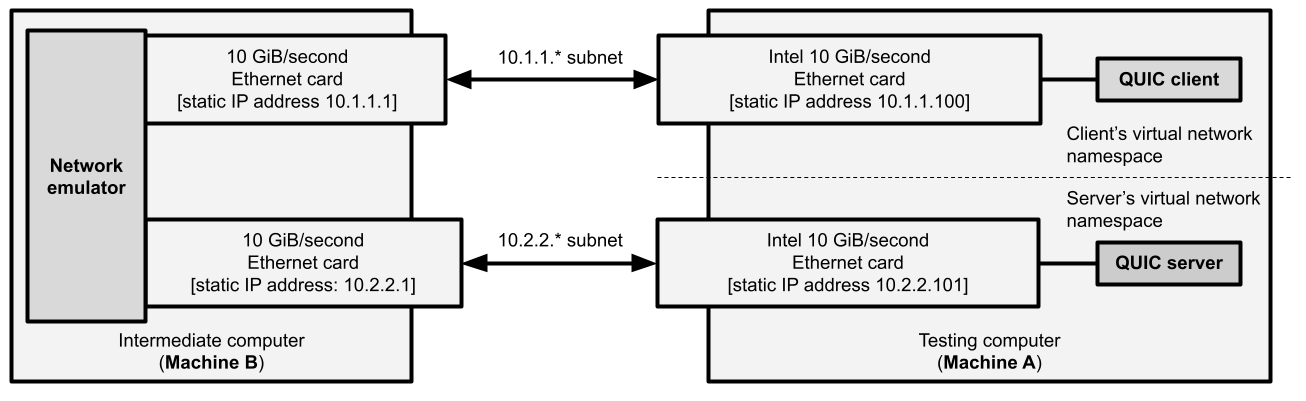
\includegraphics[width=0.9\textwidth]{figs/Physical_testing_environment.png}
    \caption{Physical configuration of testing environment}
    \label{fig:Physical_testing_environment}
    \end{figure}
    
    As we can see from Figure~\ref{fig:Physical_testing_environment}, both QUIC client and server operate on different virtual network namespaces which do not have a shared localhost/loopback [TODO check the actual name] connection.
    Client and server are assigned different network subnets.
    An intermediate machine (B) is configured as default the gateway for both virtual network namespaces.
    As a result, all the packets between the QUIC server and client have to travel via an intermediate machine (B).
    Here, depending on the experiment, network perturbations (e.g. packet loss, delay, reordering) may be introduced.
    IP forwarding is enabled on the intermediate machine (B), redirecting QUIC packets from one subnet to another.



\section{Parameter Tuning}

\subsection{IP Version}

To make results comparable with older studies, I decided to disable IPv6 in the testing environment.
By specifying a particular IP version, we reduce the number of variable parameters.
Fortunately, at the time of writing, according to Google's IPv6 adoption tracker \cite{IPv6_Adoption_Statistics}, only a third of all Internet users (30-35 \% to be precise) use IPv6 to connect to Google's services.
Hence, analysis involving IPv4 is still relevant today.

\subsection{Hyper-threading}

As Michael E. Thomadakis states on the 23rd page of \cite{hyperthreading_book}, \texttt{hyper-threading} (more generally known as \texttt{simultaneous multi-threading}) is a thread allocation technique that allows two threads to run on the same physical core at the same time.
On my particular testing machines, \texttt{hyper-threading} is implemented by assigning two virtual cores for every physical core.
As stated in \cite{hyperthreading_book}, this means that threads allocated to such virtual cores would share the same physical resources (e.g. private L1 cache entries).
This is problematic for precise experiments.
On the one hand, a neighbouring thread might pre-fetch required data to the cache, but on the other hand, this thread might pollute the cache, thus hurting the performance of the thread which is being measured.
Hence, to reduce the potential performance variability, I had to disable \texttt{hyper-threading} on the testing machines.


\subsection{Separated Cores}
Machine A in Figure~\ref{fig:Physical_testing_environment} has 4 physical cores.
To make performance tests even more predictable, I had to assign exclusive physical cores to the QUIC client and server using \texttt{taskset}\footnote{https://man7.org/linux/man-pages/man1/taskset.1.html} tool.
In particular, \texttt{ngtcp2} server was assigned the first core, QUIC client (i.e. \texttt{ngtcp2} or \texttt{h2load} client) was assigned the second core while remaining two cores were assigned to all the remaining system processes.
Robert Love refers to this technique of assigning particular processes to particular cores as \texttt{hard CPU affinity} \cite{CPU_Affinity}.

% TODO add a chart showing better throughput when using different cores for testing


% TODO add a chart showing lower performance variability when using different cores for testing



\subsection{GSO}
\begin{itemize}
  \item TODO introduce GSO
  \item TODO add a chart showing GSO's impact on throughput
  \item TODO mention when GSO is relevant
\end{itemize}

\subsection{MTUs}
\begin{itemize}
  \item TODO introduce/refresh MTUs
  \item TODO demonstrate the Jumbo frames impact for QUIC throughput
  
  
  See Table~\ref{fig:Impact_of_Jumbo_frames_for_ngtcp2_throughput}.
  
  
  
% Please add the following required packages to your document preamble:
% \usepackage{multirow}
\begin{table}[ht]

    \begin{tabular}{|c|c|c|c|c|c|}
    \hline
    \multirow{2}{*}{MTU (B)} & \multirow{2}{*}{\begin{tabular}[c]{@{}c@{}}Requested\\ file size\end{tabular}} & \multicolumn{4}{c|}{Throughput (MiB/s)}                                                     \\ \cline{3-6} 
                             &                                                                                & minimum & maximum & mean    & \begin{tabular}[c]{@{}c@{}}standard \\ deviation\end{tabular} \\ \hline
    \multirow{2}{*}{1280}    & 1MB                                                                            & 40.610  & 47.870  & 44.125  & 2.487                                                         \\ \cline{2-6} 
                             & 1GB                                                                            & 98.990  & 105.200 & 103.950 & 1.794                                                         \\ \hline
    \multirow{2}{*}{1500}    & 1MB                                                                            & 42.060  & 50.220  & 45.382  & 2.547                                                         \\ \cline{2-6} 
                             & 1GB                                                                            & 107.920 & 110.820 & 110.001 & 0.942                                                         \\ \hline
    \multirow{2}{*}{9000}    & 1MB                                                                            & 37.300  & 46.950  & 39.750  & 2.727                                                         \\ \cline{2-6} 
                             & 1GB                                                                            & 135.940 & 141.500 & 139.616 & 1.852                                                         \\ \hline
    \end{tabular}


    \begin{tabular}{|c|c|c|c|c|c|}
    \hline
    \multirow{2}{*}{MTU (B)} & \multirow{2}{*}{\begin{tabular}[c]{@{}c@{}}Requested\\ file size\end{tabular}} & \multicolumn{4}{c|}{Completion time (s)}                                                 \\ \cline{3-6} 
                             &                                                                                & minimum & maximum & mean  & \begin{tabular}[c]{@{}c@{}}standard\\ deviation\end{tabular} \\ \hline
    \multirow{2}{*}{1280}    & 1MB                                                                            & 0.020   & 0.023   & 0.022 & 0.001                                                        \\ \cline{2-6} 
                             & 1GB                                                                            & 9.070   & 9.640   & 9.180 & 0.166                                                        \\ \hline
    \multirow{2}{*}{1500}    & 1MB                                                                            & 0.019   & 0.023   & 0.021 & 0.001                                                        \\ \cline{2-6} 
                             & 1GB                                                                            & 8.610   & 8.840   & 8.674 & 0.075                                                        \\ \hline
    \multirow{2}{*}{9000}    & 1MB                                                                            & 0.020   & 0.026   & 0.024 & 0.001                                                        \\ \cline{2-6} 
                             & 1GB                                                                            & 6.740   & 7.020   & 6.834 & 0.092                                                        \\ \hline
    \end{tabular}




    \centering
    \caption{Impact of Jumbo frames on the throughput of \texttt{ngtcp2} Completion time required to transfer specified files. In particular, this experiment measures QUIC throughput between the server and the client when they are pinned to two different cores on the same machine, and their packets travel via an intermediate machine (as demonstrated in Figure~\ref{fig:Physical_testing_environment}).
    Furthermore, a server uses a single thread, only a single stream is used, and a single file transfer is performed for each experiment.
    }
    \label{fig:Impact_of_Jumbo_frames_for_ngtcp2_throughput}
\end{table}






























  
  
  
  \item TODO show that Jumbo frames are not accepted in the wild Internet
\end{itemize}


\section{Benchmarking tools}
% Frame pointer points to the top/bottom of the stack (from https://www.youtube.com/watch?v=nXaxk27zwlk&ab_channel=CppCon)

\subsection{Wireshark}

\subsection{perf}

\subsection{Flame charts}
    \begin{figure}[ht]
    \centering
    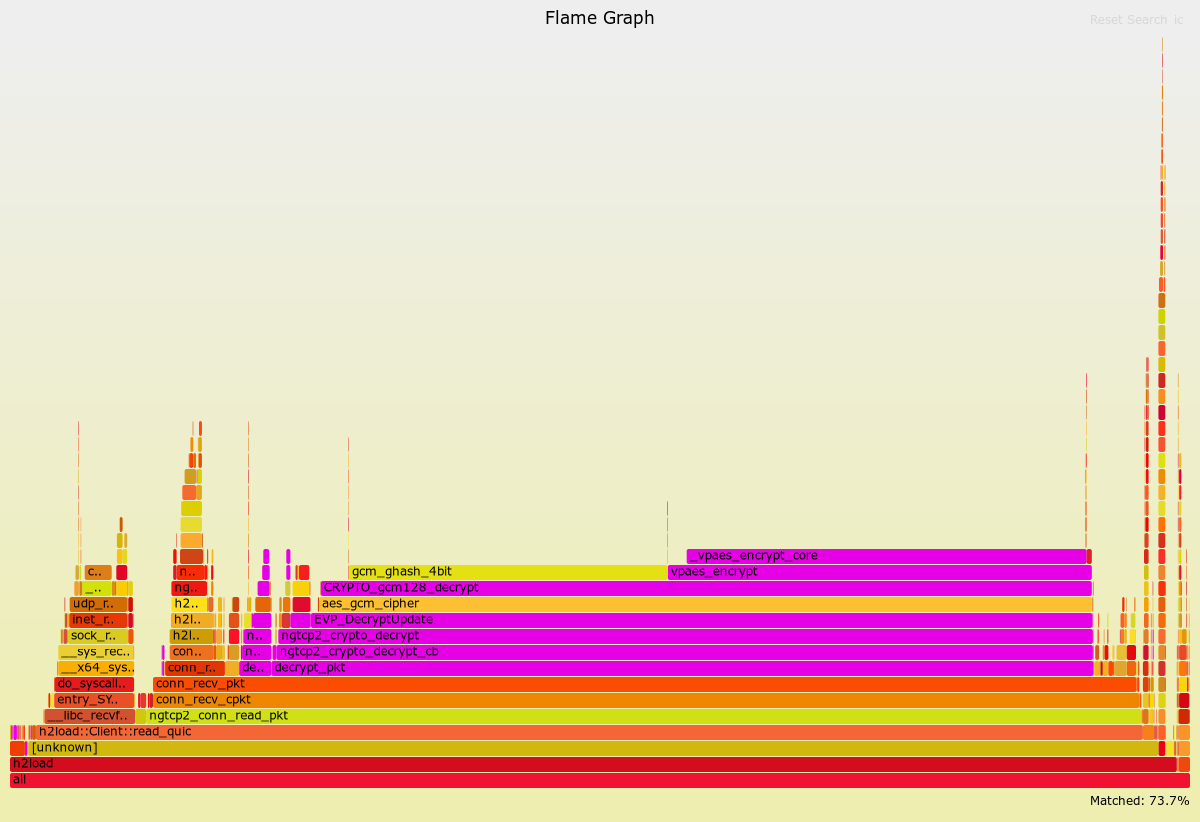
\includegraphics[width=0.9\textwidth]{figs/perf_results_of_h2load.png}
    \caption{Typical \texttt{perf} results of running \texttt{h2load} client against \texttt{ngtcp2} server on the same machine (A), when packets are transferred via an intermediate machine (B). This graph shows that about 70\% of all ngtcp2 operations are performed doing cryptographic operations} 
    \label{fig:perf_results_of_h2load}
    \end{figure}
    
\subsection{qlog}

\subsection{qvis}

\section{Impact of Cryptographic Operations}

\section{Comparison with TCP}



\chapter{Conclusion}
% ------------------------------------------------
%This chapter is likely to be very short and it may well refer back to the Introduction. It might offer a reflection on the lessons learned and explain how you would have planned the project if starting again with the benefit of hindsight.


% FROM: https://www.cst.cam.ac.uk/teaching/part-ii/projects/assessment
%Clearly presented argument demonstrating success criteria met.
%Good or excellent evidence of critical thought and interpretation of the results which substantiate any claims of success, improvements or novelty.
%Conclusions provide an effective summary of work completed along with good future work.
%Personal reflection on the lessons learned.
% ------------------------------------------------

\section{Summary}

\section{Reflection}

\section{Future Work}

%%%%%%%%%%%%%%%%%%%%%%%%%%%%%%%%%%%%%%%%%%%%%%%%%%%%%%%%%%%%%%%%%%%%%
% the bibliography
\addcontentsline{toc}{chapter}{Bibliography}
\bibliography{refs}

%%%%%%%%%%%%%%%%%%%%%%%%%%%%%%%%%%%%%%%%%%%%%%%%%%%%%%%%%%%%%%%%%%%%%
% the appendices
\appendix

\chapter{Source A}


\chapter{Source B}

\section{appendix section}\label{referencedAppendixTag}


\chapter{Project Proposal}

\documentclass[a4paper,12pt]{article}
\usepackage[utf8]{inputenc}
\usepackage[british,UKenglish]{babel}
\usepackage{enumitem}
\usepackage{parskip}
\usepackage{csquotes}
%opening

\begin{document}

% This is all copied from the diploma one and honestly it's disgusting
\leftline{\large\emph{Candidate Number:              2439D}}
\medskip
\leftline{\large\emph{College: Homerton College}}

\vfil

\centerline{\large Computer Science Tripos Part II Project Proposal}
\vspace{0.4in}
\centerline{\Large \textbf{QUIC offloading using NetFPGA smart NIC}}
\vspace{0.3in}
\centerline{\large \today}

\vfil

\textbf{Project Originator:} Dr Andrew W. Moore

\vspace{0.5in}

\textbf{Project Supervisor:} Dr Andrew W. Moore

\vspace{0.2in}

{\bf Signature:}

\vspace{0.5in}

{\bf Director of Studies:} Dr John Fawcett 

\vspace{0.2in}

{\bf Signature:}

\vspace{0.5in}

{\bf Overseers:} Dr Robert Mullins and Dr Marcelo Fiore

\vspace{0.2in}

{\bf Signatures:}

\vfil
\eject

\section*{Introduction and Description of the Work}
QUIC is a new transport layer protocol built on top of UDP.
QUIC has numerous advantages compared to TCP: 
QUIC establishes connections faster, 
it aims to prevent ossification of network standards by encrypting network headers 
and	QUIC's multiplexed connections don't suffer from the head-of-line blocking.
Some implementations of QUIC provide a mechanism to fall back to TCP if QUIC is not supported by either of the communicating parties or an intermediate network infrastructure (e.g. firewalls).
This detection mechanism is done in parallel, so QUIC should be no worse than TCP.
Despite these advantages, for historical reasons, TCP has better hardware support than QUIC.
For example, QUIC requires 350\% more CPU cycles than TCP with TLS [1].
The reason for such a clear difference is that in the last years TCP/IP network stack was considered to be the backbone protocol of the Internet.
As a result, multiple middleboxes and hardware accelerators were created to support and enhance TCP.

In contrast, QUIC doesn't have widespread hardware support as it is a new and developing standard.
Consequently, there is a risk that because of this lack of support, QUIC may not be adopted.
To mitigate this issue, I am planning to do partial QUIC offloading with smart NICs on the receiver's side.
In other words, the goal of this project is to delegate some CPU intensive but primitive tasks to hardware, leaving more complex control operations to CPU.

There is an increasing workload pressure for CPUs as network throughput keeps increasing.
Processors need to perform expensive context switch operations to handle incoming packets.
For instance, CPUs may perform cryptographic operations on packets, and they usually reply with acknowledgements.
Contention for CPUs can be relieved by delegating specific instructions to NICs (network interface cards).

Studies show that after encryption packet reordering is another bottleneck of QUIC[2].	
My core goal is to create packet reordering logic in hardware using NetFPGA-SUME smart NIC.
However, by design QUIC encrypts packet numbers so this project would require me to turn off encryption of QUIC. 
In case it turns out to be impossible, I am planning to offload packet pacing functionality to Net-FPGA SUME board.

If time allows, I am planning to implement additional offloading functions in hardware.
For example, potential extension goal is to implement QUIC packet segmentation in hardware.
Another additional task could be to offload QUIC encryption and/or decryption functions to hardware.

I am planning to provide some semi-random stimulus to the test logic. 
I would have to test that offloaded logic correctly deals with both correct and malformed QUIC packets. 
As a result, I should randomise payload of the potential packets to have representative inputs. 
Moreover, the random stimulus can be tested in both the application layer and in hardware (NetFPGA NIC). 
Application layer testing would require an end-to-end testing environment of two machines which would be using QUIC for communication. 
Random message contents or random lengths could be exchanged to ensure that my offloading logic does not introduce new errors. 
Hardware-level testing could be performed in isolation analysing the behaviour of FPGAs. 
This project is concerned with partial offloading so my offloading logic shouldn’t make any complicated control decisions (e.g. CPU would have to deal with the complicated task of removing unsuitable QUIC packets). 
Hence, packet reordering should not change the size of incoming data. 
As a result, I could add additional supervising logic to ensure that this property is preserved. 

\section*{Starting Point}
This project will use insights from other researchers who investigated the possibility of QUIC offloading [2] and who actually offloaded cryptographic functions [7].
Moreover, a similar part II project was done in the past with a different transport layer protocol (TCP) [4].
My initial project will be built on top of the NetFPGA SUME template for building network interface cards (NICs) [6].

To simplify FPGA debugging process, I am planning to make use of numerous network debugging tools. 
First of all, qvis can be used to represent logs of QUIC graphically.  
Moreover, the NetFPGA SUME board uses Xilinx software which includes Vivado simulator.  
Finally, it seems that packet manipulation tool Scapy could be used for testing as well.  
 
As far as network simulation is concerned, it seems that TLEM network emulator [8] could be used for integration testing. TLEM has already been used in the paper which compared different implementations of QUIC [2]. Hence, I assume that I could also make use of this emulator. 

\section*{Essential Tasks to be completed}

The core goal can be split into multiple sub-tasks:
\begin{itemize}
  \item 
First of all, I will need to construct an initial hardware component which could retrieve the relevant information (such as connection ID) from QUIC headers. 
According to [3], all the QUIC packets, including packet numbers, are encrypted.
Hence, I would need to find a mechanism which would allow me to turn off encryption.
If that doesn't work, then I will have to create my own simplified version of unencrypted QUIC protocol.
For this reason, I can't tell which implementation of QUIC I will be using during the development time.

  \item 
Later on, relevant packet information will be used to group and place packets into the buffers. 
Each connection should have its own dedicated buffer. 
It turns out that there is no buffer memory manager, so I would have to create one myself. 
Moreover, I anticipate that I would have to implement an additional layer which would enable communications between the current QUIC implementations and my underlying offloading hardware. 
This task would require special attention when dealing with concurrency.
Hardware analogues of test-and-set instructions or spin-locks might be useful here.

  \item 
Additionally, I would need to create a timestamp generator and/or some ``garbage collector" so that I could remove lost or outdated packets.
I found that a former part II student observed abnormal behaviour of Enthernet's TX and RX clocks in his Part II dissertation [4].
My current knowledge allows me to assume that this issue is irrelevant as I would be using a separate system clock.
 \end{itemize}

\section*{Extended goals}
 If time allows, I should implement the following tasks:
 \begin{itemize}
  \item offload QUIC packet segmentation to hardware
  \item offload QUIC encryption and/or decryption to hardware
 \end{itemize}

\section*{Success Criteria}
To demonstrate the success of my project, I would have to test my implementation of packet reordering mechanism.
To do this, I will have to write unit tests which would show that my logic is capable of dealing with different (e.g. non-standard or corrupt) packets. 
If it turned out that it was impossible to overcome QUIC encryption, but I implemented and tested packet pacing logic, then my project would still be considered a success.

In addition to numerous unit tests, I could also use interoperability tests to ensure that offloaded core functions of QUIC still work.
Unfortunately, I am planning to use QUIC in a non-standard way (without encryption), so interoperability tests would not be relevant.

A further success criterion is to obtain quantitative performance metrics of my implementation.
I should compare two network stacks: one which uses QUIC and another which uses QUIC with hardware offloading.
It will be sufficient to measure delay, throughput and the number of CPU cycles consumed by each stack when sending data between two connected machines. 
Also, associated costs of offloading (used FPGA area and processing time of packets) should be included in the final report.
I expect that this experiment would demonstrate that my implementation could reduce the number of required CPU cycles to process QUIC packets.

However, it is highly likely that clocks of different machines will be skewed. Even the smallest difference in time could change performance metrics. 
To mitigate this issue, I could change the message path – all the packets would have to go from sender to receiver and then back again to the sender. 
Alternatively, I would have to measure an upper boundary for the clock skew, and I would have to take it into account when reporting my findings. 




\section*{Timetable and Milestones}
In order to be able to track my progress, I am planning to split my work into slots of 14 days.
It seems reasonable to start each work item on Saturday and finish it after two weeks on Friday because various deadlines will be on Fridays.

% \begin{enumerate}[label=\textbf{Slot \arabic*} -,start = 1]
 \begin{enumerate}
  \item \emph{24th October -- 6th November}

\textbf{Tasks}
 \begin{itemize}
  \item Create a testing environment where two processes on different Virtual Machines would exchange QUIC packets.
  \item Finish tutorial (provided by https://netfpga.org/) about NetFPGA SUME boards.
  \item Obtain required special hardware and set up a development environment.
 \item Read papers about offloading techniques used for TCP and QUIC.
 \item Find a mechanism to turn off QUIC encryption or find QUIC implementation which doesn't have it.
  If that turns out to be impossible, then I would have to propose minimal requirements to implement my own version of QUIC. 
 \end{itemize}


\textbf{Milestone}
 \begin{itemize}
  \item Produce and send a report to the project supervisor about the key functionality of NetFPGA SUME boards, TCP and QUIC offloading and propose a strategy to get rid of QUIC encryption.\\
\emph{Due 6th November.}
 \end{itemize}
 
\textbf{Course work deadlines}
 \begin{itemize}
  \item Unit of assessment practical work deadline -- 27th October.
 \end{itemize} 




 \item 
 \emph{7th November -- 20th November}

\textbf{Tasks}
 \begin{itemize}
  \item 
  Remove the encryption from QUIC packets. 
  This can be done by either using QUIC an implementation which allows that, adjusting encryption module or creating a minimal version of my own QUIC implementation which doesn't have encryption.
  \item 
  Create hardware component which would retrieve packet number.
 \item 
  Write unit tests for this hardware component.
 \item 
  (Extra) Study documentation of Vivado simulator and packet manipulation tool Scapy.
 \end{itemize}

\textbf{Milestone}
 \begin{itemize}
  \item 
  Remove encryption and implement simple hardware module which extracts QUIC packet numbers.
 \item 
  (Extra) Create a short report about Vivado simulator and Scapy.
 \emph{ Due 20th November. }
 \end{itemize}

 \textbf{Course work deadlines}
 \begin{itemize}
  \item 
  Unit of assessment practical work deadline -- 10th November.
 \end{itemize} 



 
 \item 
 \emph{21st November -- 4th December}

\textbf{Tasks}
 \begin{itemize}
  \item
   Finish removal of encryption if there are any unexpected difficulties.
  \item 
  Check if it is possible to use Xilinx software licences outside the Cambridge network.
  \item 
  Set up a working environment so that it could be accessed remotely.
 \end{itemize}

\textbf{Milestone}
 \begin{itemize}
  \item 
  Have a prepared remote working environment.
  Moreover, at this point, I should have removed encryption from QUIC and implemented simple hardware module which extracts QUIC packet numbers.\\
 \emph{ Due 4th December.}
 \end{itemize}

 \textbf{Course work deadlines}
 \begin{itemize}
  \item 
  Unit of assessment report submission deadline -- 3rd December.
 \end{itemize} 
 




 \item 
 \emph{5th December -- 18th December}

 \textbf{Tasks}
 \begin{itemize}
  \item Implement Verilog block which would generate timestamps.
  \item Write Verilog code which would store QUIC packets in registers.
  \item Implement unit tests which would ensure the correctness of these blocks.
  \item Read about the concurrent-safe hardware operations available in Net FPGA SUME boards.
 \end{itemize}

\textbf{Milestone}
 \begin{itemize}
  \item Have a working Verilog code which would order QUIC packets.\\
  \emph{ Due 18th December. }
 \end{itemize}
 



 \item 
 \emph{19th December -- 1st January}

 \textbf{Tasks}
 \begin{itemize}
  \item Start working on the integration of QUIC offloading with actual QUIC protocol.
  \item Continue developing previous Verilog items if I encounter any unexpected difficulties.
 \end{itemize}

\textbf{Milestone}
 \begin{itemize}
  \item Have a working Verilog code which would order QUIC packets. Also, at this point, I should have successfully integrated QUIC offloading with QUIC protocol.
Also, I should send an update of my progress to the supervisor.\\
 \emph{ Due 1st January. }
 \end{itemize}
 


 \item 
 \emph{2nd January -- 15th January}

 \textbf{Tasks}
 \begin{itemize}
   \item Catch up with any unexpected difficulties.\\
 \end{itemize}

\textbf{Milestone}
 \begin{itemize}
   \item Send an update of my progress to the supervisor.\\
 \emph{ Due 15th January. }
 \end{itemize}

 


 \item 
 \emph{16th January -- 29th January}

\textbf{Tasks}
 \begin{itemize}
  \item Create end-to-end integration testing environment.
  \item Create simulation environment which would delay and reorder packets according to the specified parameters.
  \item Start measuring offloading performance.

 \item If time allows, then start working on extensions.
 \item Continue measuring offloading performance.
 \end{itemize}

\textbf{Milestone}
 \begin{itemize}
  \item Measure throughput and latency of offloaded QUIC protocol using different size packets and network conditions.
  \item Measure CPU usage of the offloaded QUIC protocol.
  \item Measure consumed FPGA area and processing time of packets.\\
 \emph{ Due 29th January. }
 \end{itemize}
  



 \item 
 \emph{30th January -- 12th February}

\textbf{Tasks}
 \begin{itemize}
 \item Start working on the progress report and its presentation.
 \end{itemize}

\textbf{Milestone}
 \begin{itemize}
  \item Send progress report before the deadline.
  \item Finish progress report presentation.\\
 \emph{ Due 12th February. }
 \end{itemize}

 \textbf{Deadlines}
 \begin{itemize}
  \item Progress Report Deadline -- 5th February, 12 noon.
  \item Progress Report Presentations -- 11th, 12th, 15th or 16th February, 2:00 PM.
 \end{itemize}

 \textbf{Course work deadlines}
 \begin{itemize}
  \item Unit of assessment assignment deadline -- 1st February.
 \end{itemize} 
 



 \item 
 \emph{13th February -- 26th February}

\textbf{Tasks}
 \begin{itemize}
 \item If time allows, continue working on extensions.
 \item Otherwise, perform more evaluation tests.
 \end{itemize}

\textbf{Milestone}
 \begin{itemize}
  \item Send progress update to the project supervisor.\\
 \emph{ Due 26th February. }
 \end{itemize}

 \textbf{Course work deadlines}
 \begin{itemize}
  \item Unit of assessment assignment deadline -- 15th February.
 \end{itemize} 



 
 \item 
 \emph{27st February -- 12th March}

\textbf{Tasks}
 \begin{itemize}
 \item If time allows, write unit tests for extensions.
 \item Otherwise, finish evaluation testing.
 \end{itemize}

\textbf{Milestone}
 \begin{itemize}
  \item Send conclusions of evaluation to the project supervisor.\\
 \emph{ Due 12th March. }
 \end{itemize}

 \textbf{Course work deadlines}
 \begin{itemize}
  \item 
  Unit of assessment report deadline -- 12 March.
 \end{itemize} 
 




 \item 
 \emph{13th March -- 26th March}

 \textbf{Tasks}
 \begin{itemize}
  \item 
  Write a chapter about introduction and preparation.
 \end{itemize}

\textbf{Milestone}
 \begin{itemize}
  \item Send introductory chapters to the project supervisor.\\
 \emph{ Due 26th March.}
 \end{itemize}




 \item 
 \emph{27th March -- 9th April}

\textbf{Tasks}
 \begin{itemize}
 \item Adjust previous chapters to the comments from the supervisor.
 \item  Write a chapter about implementation.
 \end{itemize}

\textbf{Milestone}
 \begin{itemize}
  \item Send implementation chapters to the project supervisor.\\
 \emph{ Due 9th April. }
 \end{itemize}
 




 \item 
 \emph{10th April -- 23rd April}

 \textbf{Tasks}
 \begin{itemize}
  \item 
  Adjust previous chapters to the comments from the supervisor.
 \item 
  Write evaluation chapter.
 \end{itemize}


\textbf{Milestone}
 \begin{itemize}
  \item Send draft version of dissertation to the project supervisor and Director of Studies.\\
 \emph{ Due 23rd April. }
 \end{itemize}



 
 \item 
 \emph{24th April -- 7th May}

 \textbf{Tasks}
 \begin{itemize}
  \item Adjust dissertation to the comments from the supervisor and Director of Studies.
 \end{itemize}

\textbf{Milestones}
 \begin{itemize}
  \item Send final version of dissertation to the supervisor and Director of Studies.
  \item Submit dissertation before the deadline.
 \emph{ Due 7th May. }
 \end{itemize}






\item 
 \emph{8th May -- 14th May}
 
 \textbf{Tasks}
 \begin{itemize}
  \item Ensure that the dissertation is submitted a few days before the deadline.
 \end{itemize}


\textbf{Milestone}
 \begin{itemize}
  \item Have a submitted dissertation.\\
 \emph{ Due 14th May. }
 \end{itemize}

 \textbf{Deadlines}
 \begin{itemize}
  \item 
  Dissertation Deadline -- 14th May, 12 noon.
  \item
  Source Code Deadline -- 14th May, 5:00 PM.
 \end{itemize}
\end{enumerate}

\section*{Resources Declaration}
 \textbf{This project requires specific hardware resources: }
 \begin{itemize}
\item 
\textbf{Two NetFPGA SUME boards and all the required licences}\\
\textit{Contact person: Dr Andrew W. Moore (andrew.moore@cl.cam.ac.uk)}\\
These smart NICs have programmable FPGAs which would allow me to implement packet reordering logic in hardware.
Moreover, these boards have high throughput (1-10 Gbps), and there is a large NetFPGA community of developers.
According to [5], ``Current NetFPGA work is licensed under LGPL 2.1".

\item
\textbf{Two pre-build NetFPGA Cube systems}\\
\textit{Contact person: Dr Andrew W. Moore (andrew.moore@cl.cam.ac.uk)}\\
These integrated computer systems will substantially simplify the development process as they combine NetFPGA SUME boards with motherboards and additional hardware components.
Moreover, these cube systems will reduce the risk of physical damage.

\item
\textbf{Connecting Ethernet cables}\\
\textit{Contact person: Dr Andrew W. Moore (andrew.moore@cl.cam.ac.uk)}
 \end{itemize}

I am planning to use my own personal computer because of convenience and familiarity.
This is a dual-boot system with both Windows 10 Pro and Ubuntu 18.04.
My computer has Intel(R) Core(TM) i7-8550U CPU whose working frequency is 1.80GHz.
8 GB amount of RAM is dedicated for Windows partition, and there are 7.6 GB available RAM dedicated for Ubuntu partition.\\

I accept full responsibility for this machine, and I have made contingency plans to protect myself against hardware and/or software failure.
For example, I am planning to use Git for version control and upload my daily progress to a remote repository on GitHub.
Moreover, each week I will be backing up my files to Google Drive and a separate hard disk which would be used only for this purpose.
I will buy a second computer if my current machine stops working.

In case my special hardware stops working properly, I could always transition to work in the Computer Laboratory.
There are similar older generation NetFPGA boards (``NetFPGA 1G") whose network throughput is smaller (1Gbps instead of 10Gbps).

\section*{External Information Sources}

[1]
Adam Langley, Alistair Riddoch, Alyssa Wilk, Antonio Vicente, Charles Krasic,
Dan Zhang, Fan Yang, Fedor Kouranov, Ian Swett, Janardhan Iyengar, Jeff Bailey,
Jeremy Dorfman, Jim Roskind, Joanna Kulik, Patrik Westin, Raman Tenneti,
Robbie Shade, Ryan Hamilton, Victor Vasiliev, Wan-Teh Chang, and Zhongyi Shi.
2017. The QUIC Transport Protocol: Design and Internet-Scale Deployment. In
Special Interest Group on Data Communication (SIGCOMM). ACM.

[2]
Xiangrui Yang, Lars Eggert, Steve Uhlig, Zhigang Sun, Gianni Antichi.\\
2020. Making QUIC Quicker With NIC Offload\\
Figure 3 from https://dl.acm.org/doi/pdf/10.1145/3405796.3405827

[3]
https://tools.ietf.org/id/draft-ietf-quic-manageability-04.html

[4]
Eliot Lim
Part II dissertation "Performant TCP bytestreams on FPGAs"\\
https://www.cl.cam.ac.uk/teaching/projects/archive/2020/el462-dissertation.pdf, page 3.

[5]
Noa Zilberman, Yury Audzevich, G. Adam Covington and Andrew W. Moore,\\
"NetFPGA SUME: Toward 100 Gbps as Research Commodity," IEEE Micro,\\
vol.34, no.5, pp.32-41, Sept.-Oct. 2014, doi: 10.1109/MM.2014.61

[6]
https://github.com/NetFPGA/NetFPGA-SUME-public/wiki/NetFPGA-SUME-Reference-NIC

[7]
Offloading QUIC - An Implementation Guide\\
Manasi Deval, Gregory Bowers, \\
IETF 104, Prague, March 2019\\
https://www.ietf.org/proceedings/104/slides/slides-104-quic-offloading-quic-00

[8]
https://www.researchgate.net/publication/306925556\_Very\_high\_speed\_link   \_emulation\_with\_TLEM 


\end{document}


 \end{document}
